\chapter{原系统分析和重构目标}

\section{Unix V6++ 原系统概述}

Unix V6++是同济大学为操作系统课程教学而开发的实验平台，其设计思想来源于 1975 年发布的经典 Unix Version 6。该系统在保留 Unix V6 核心机制和整体结构的基础上，结合 PC 平台硬件环境，使用 C++对内核进行重新实现，使其能够运行在 IA32架构上。与现代商用的复杂操作系统相比，Unix V6++代码规模较小、模块划分清晰、运行机制完整，适合作为教学操作系统使用。从教学定位上看，Unix V6++并不追求功能完备或工程规模，而是通过较小的代码体量呈现操作系统的核心机制，包括进程管理、内存管理、文件系统、设备管理与中断处理等。学生可以在阅读和修改源码的过程中，理解操作系统各模块之间的协作关系，从而将课堂中的抽象概念与具体实现联系起来。代码结构上，Unix V6++采用较为典型的分层组织方式。系统底层由 machine、interrupt、boot 等模块组成，负责处理与 IA32 平台相关的启动、分页、中断、时钟和设备控制逻辑；中间由 proc、mm、fs、dev 等模块构成，分别对应进程管理、内存管理、文件系统和设备管理；上层则通过系统调用接口向用户程序提供运行环境。其中，boot 模块负责内核装载与启动；machine 模块管理 GDT、IDT、页表等体系结构相关对象；proc 模块实现进程控制块、调度、fork、exec 和 wait 等核心机制；mm 模块负责页式内存分配和换出管理；fs 模块实现 Unix 风格文件系统；dev 模块则通过缓冲区缓存和块设备驱动完成对外设的统一访问。整体上，该系统保留了传统Unix 的基本组织方式，具有较强的教学示范意义。

\section{原系统关键模块分析}

\subsection{内存管理机制分析}

原系统的内存管理模块主要位于 src/mm/目录下，核心类包括 PageManager、KernelPageManager、UserPageManager、KernelAllocator 和 SwapperManager。系统采用页式内存管理方式，以 4KB 为基本分页单位，对内核空间和用户空间分别维护独立的页分配区域。根据 PageManager.h 中的定义，内核页池和用户页池具有固定的起

始地址和大小，内存分配以页为单位进行。

\begin{figure}[htbp]
  \centering
  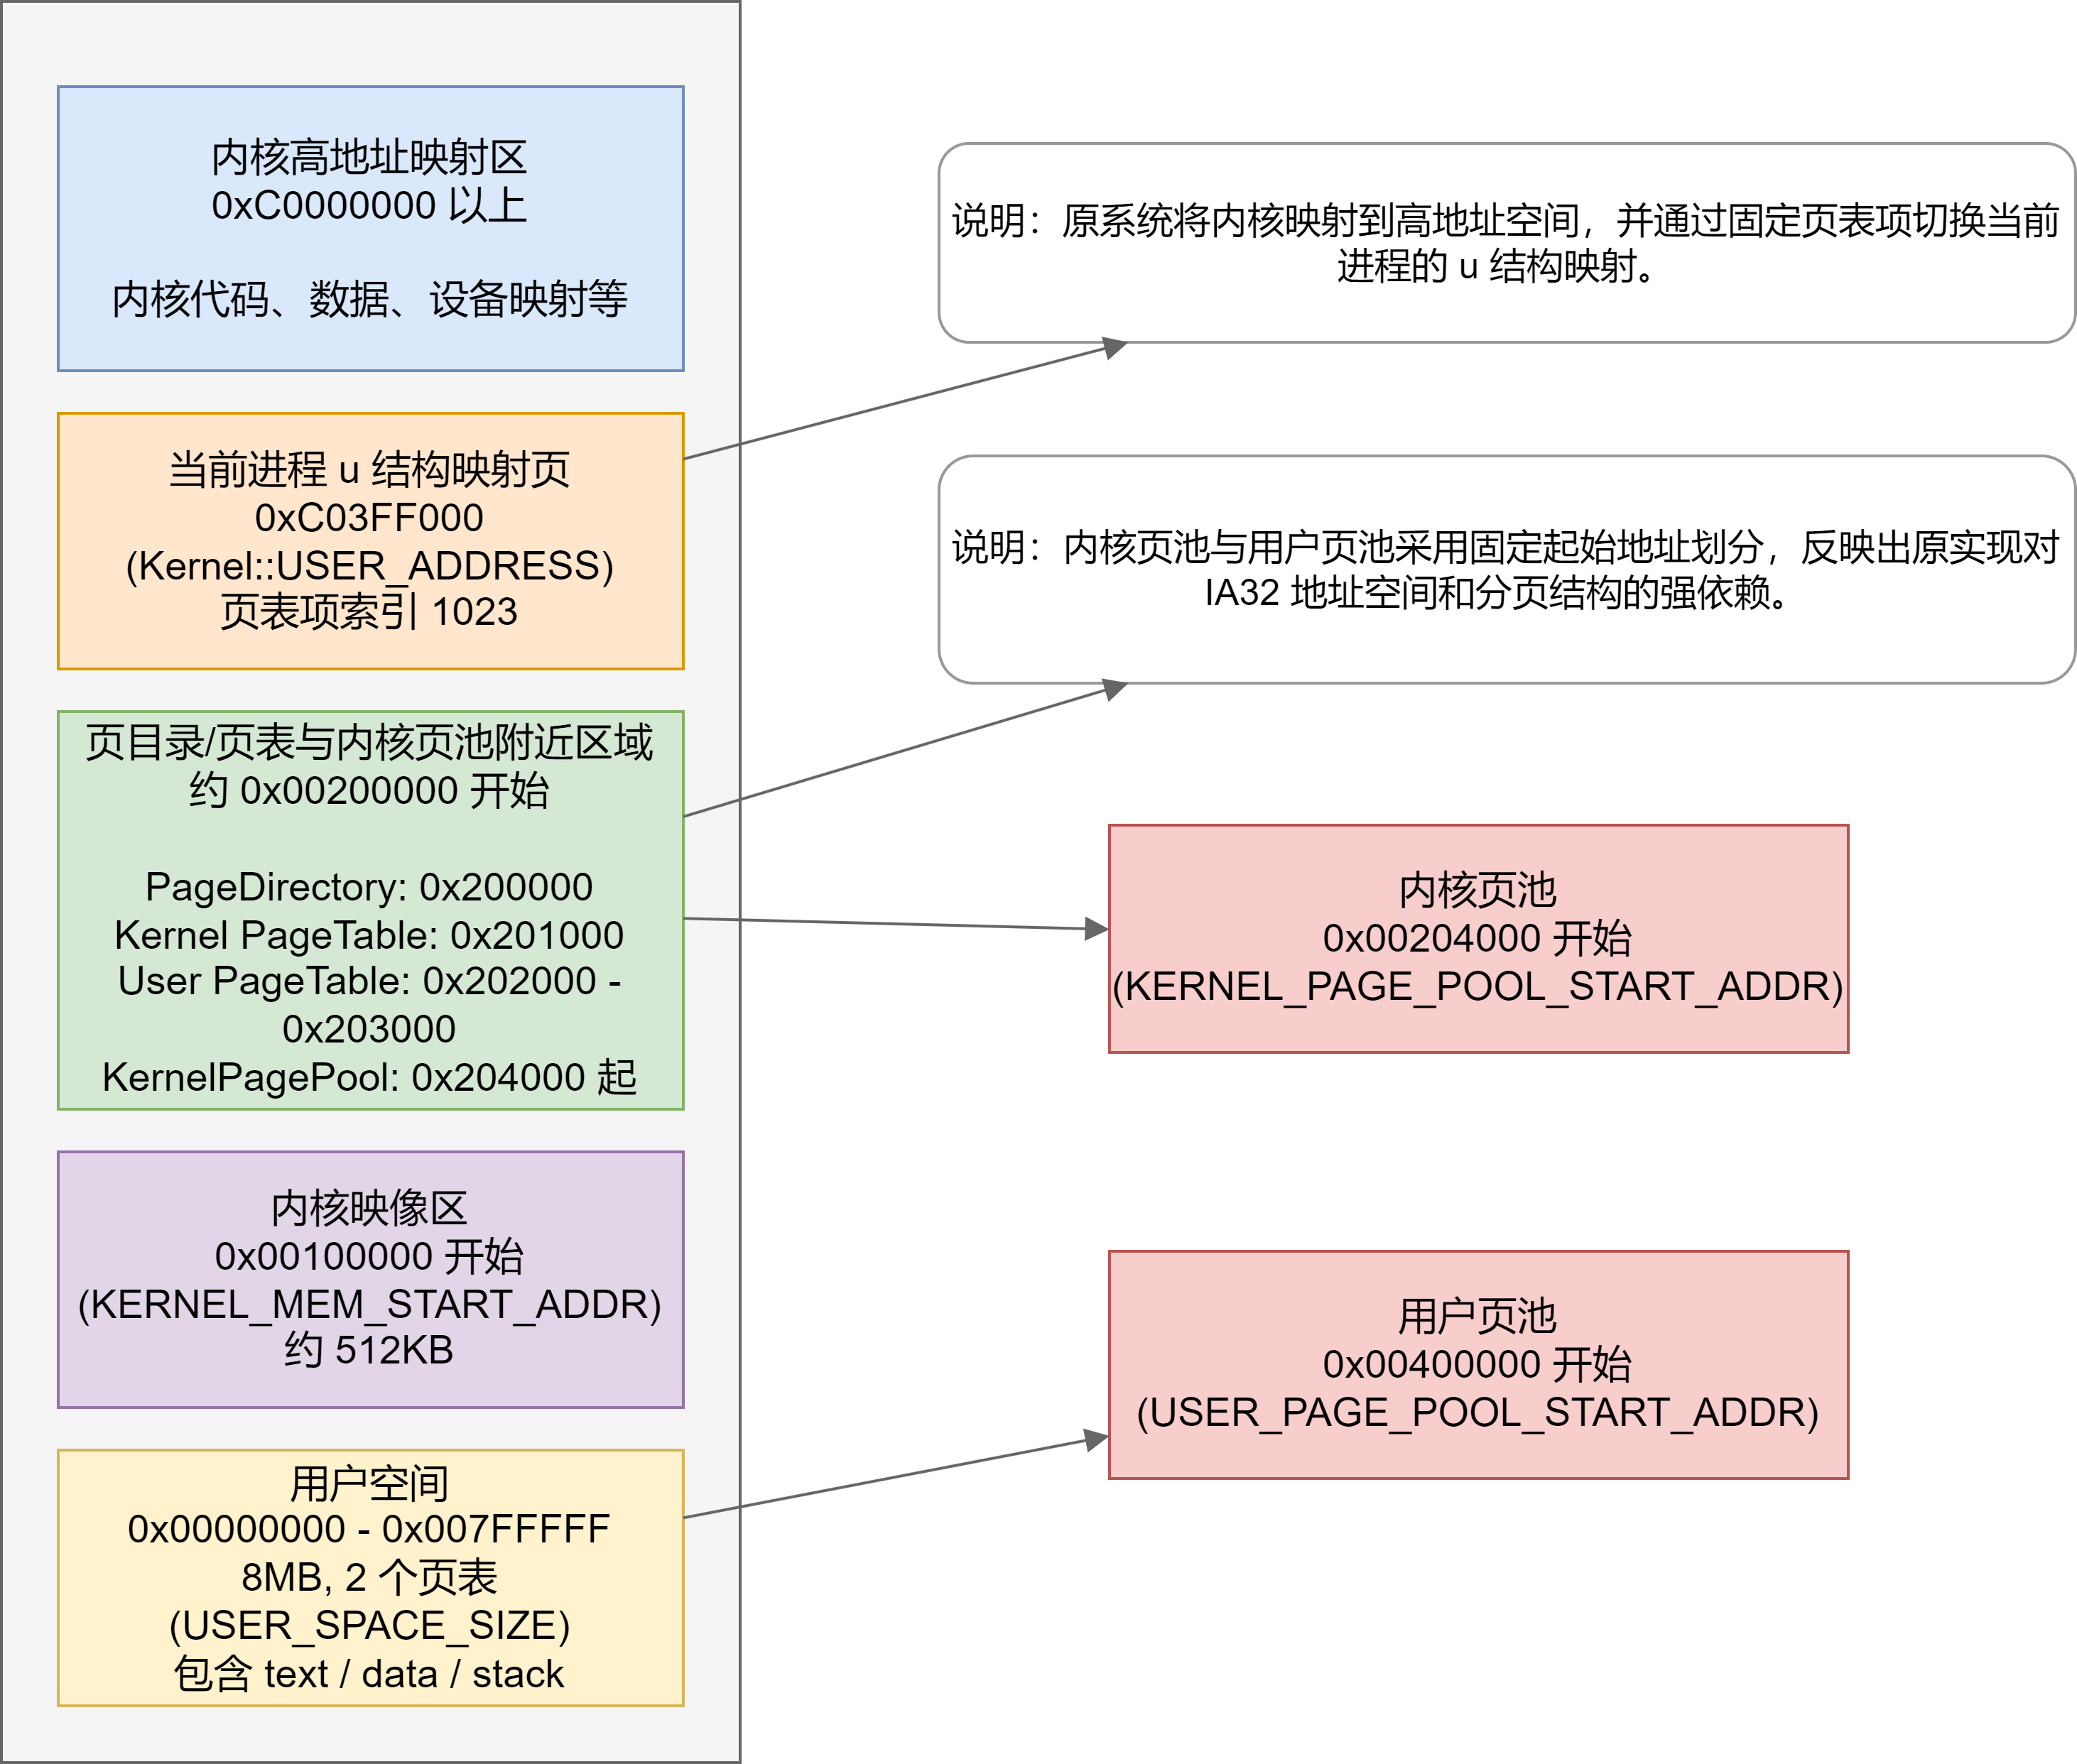
\includegraphics[width=0.74\textwidth]{figures/2/1内存布局.png}
  \caption{原系统内存布局示意图}
\end{figure}

在实现上，系统通过 MapNode 等数据结构维护可用页框的分配状态，并提供内存申请与释放接口。对于内存不足的情况，系统还提供了交换管理机制，由SwapperManager 负责在主存和交换区之间转移进程映像，以支持较为传统的 Unix 式换出策略。整体来看，原系统已经具备了教学所需的基本页式管理和交换能力，能够支撑进程运行、用户区分配和页表映射等核心功能。但是，原实现的内存分配算法相对较为简陋，主要面向教学场景下的基本可用性设计，在分配策略、碎片控制和扩展性方面都比较有限。其页分配机制为对固定内存区域的直接管理，缺少更精细化的分层分配设计，也没有适合不同大小对象的高效动态分配机制。这种实现便于学生理解基本原理，但有灵活性不足、资源利用率不高等问题。同时，该模块与 IA32 的分页结构绑定较紧，也限制了其在新架构上的直接复

用能力。

\subsection{文件系统机制分析}

原系统的文件系统模块主要由 FileSystem、INode、File、FileManager 和OpenFileManager 等部分组成，相关代码位于 src/fs/目录。系统延续了 Unix V6 的基本设计，以超级块、i 节点、目录项和数据块为核心数据结构，通过块设备组织磁盘上的文件和目录信息。从 ileSystem.h 可以看出，系统维护了超级块中的空闲数据块表和空闲 i 节点表，并通过 IAlloc、IFree、Alloc、Free 等接口管理磁盘空间与 inode 资源。文件访问流程则通过 FileManager 组织路径解析、打开、关闭、创建、链接和删除等操作，通过OpenFileManager 维护系统范围内的打开文件表。整体而言，该模块较完整地复现了传统 Unix 文件系统的组织方式，适合作为教学中的文件系统案例。

\begin{figure}[htbp]
  \centering
  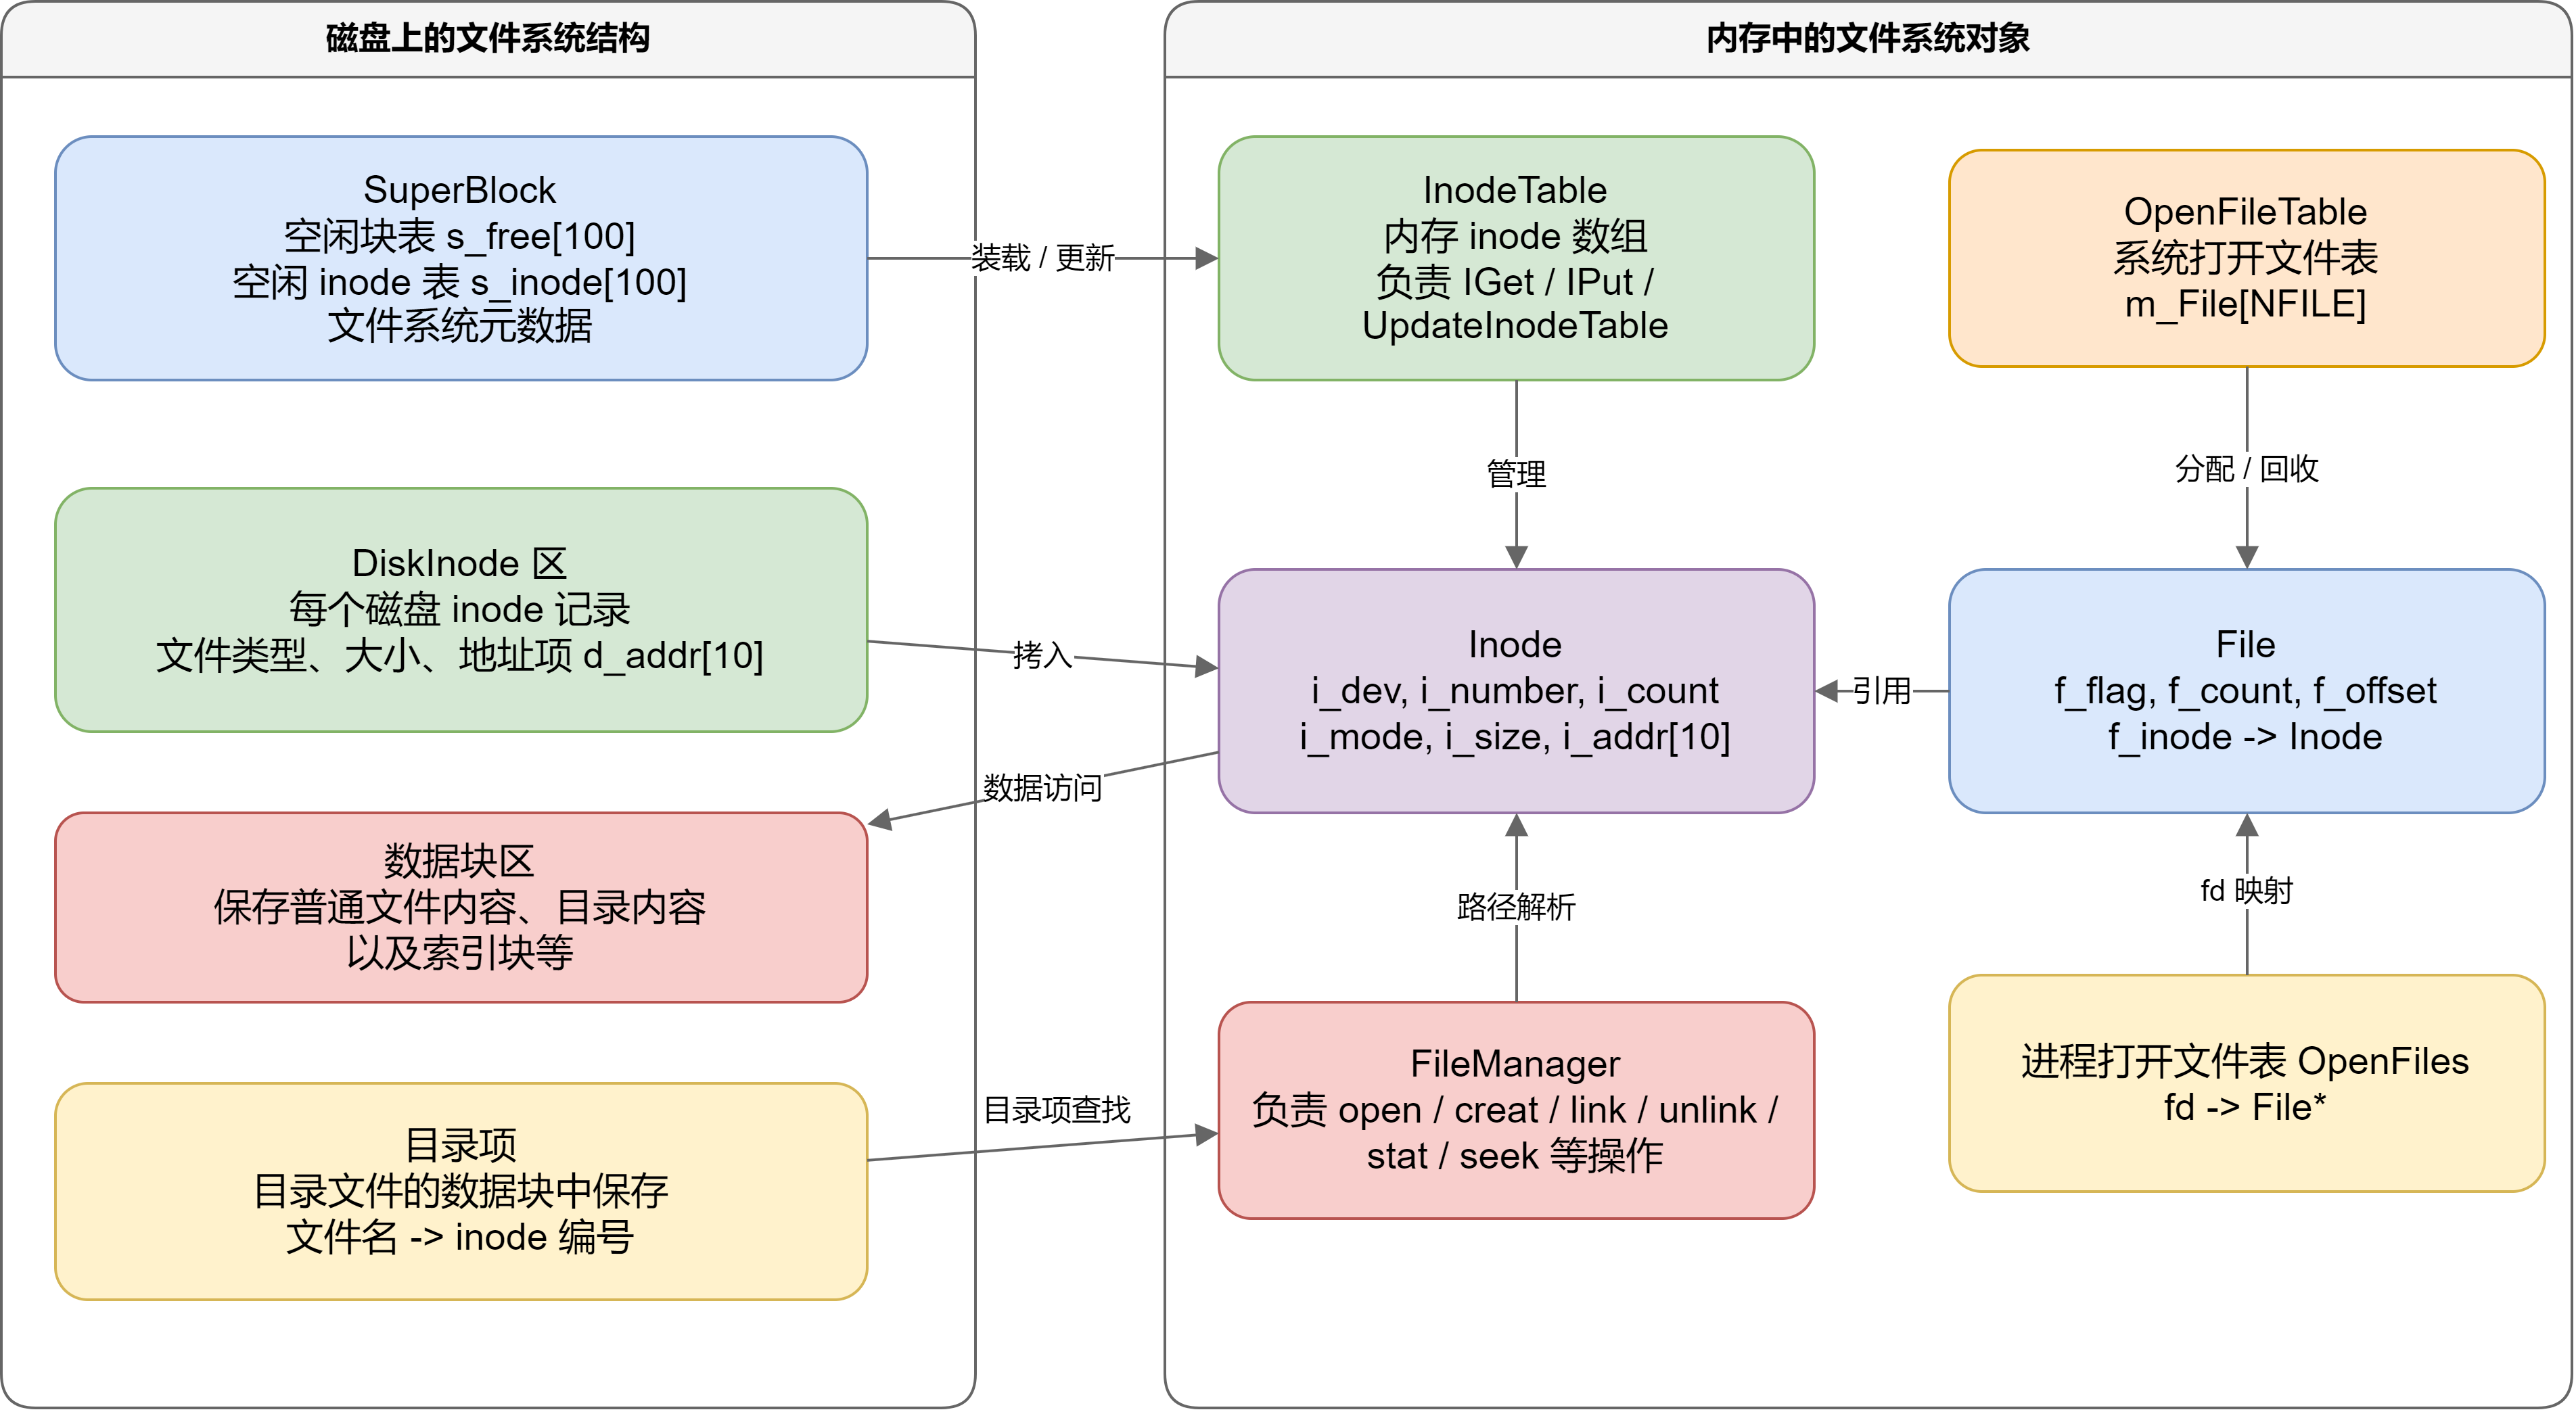
\includegraphics[width=0.72\textwidth]{figures/2/2文件系统.png}
  \caption{文件系统核心数据结构关系图}
\end{figure}

\subsection{缓冲区缓存与设备管理机制分析}

原系统的缓冲区缓存与设备管理机制主要位于 src/dev/目录中，核心包括BufferManager、Buf、DeviceManager、BlockDevice、CharDevice 和 ATADriver 等部

分。系统采用缓冲区缓存作为块设备访问的中间层，以减少对底层磁盘的直接访问频率，并统一文件系统与设备层之间的数据交换接口。

根据 BufferManager.h 的定义，系统维护固定数量的缓冲区控制块和数据区，通过 GetBlk、Bread、Bwrite、Brelse 等接口支持同步读写、预读、延迟写和异步写等操作。设备管理部分通过 DeviceManager 对不同类型设备进行组织，其中块设备访问最终由 ATADriver 完成，驱动层直接操作 IA32 平台上的 I/O 端口和 ATA 控制器寄存器，实现扇区级数据传输。是比较经典的文件系统 - 缓冲区缓存 - 块设备驱动的 UnixI/O 路径。

\begin{figure}[htbp]
  \centering
  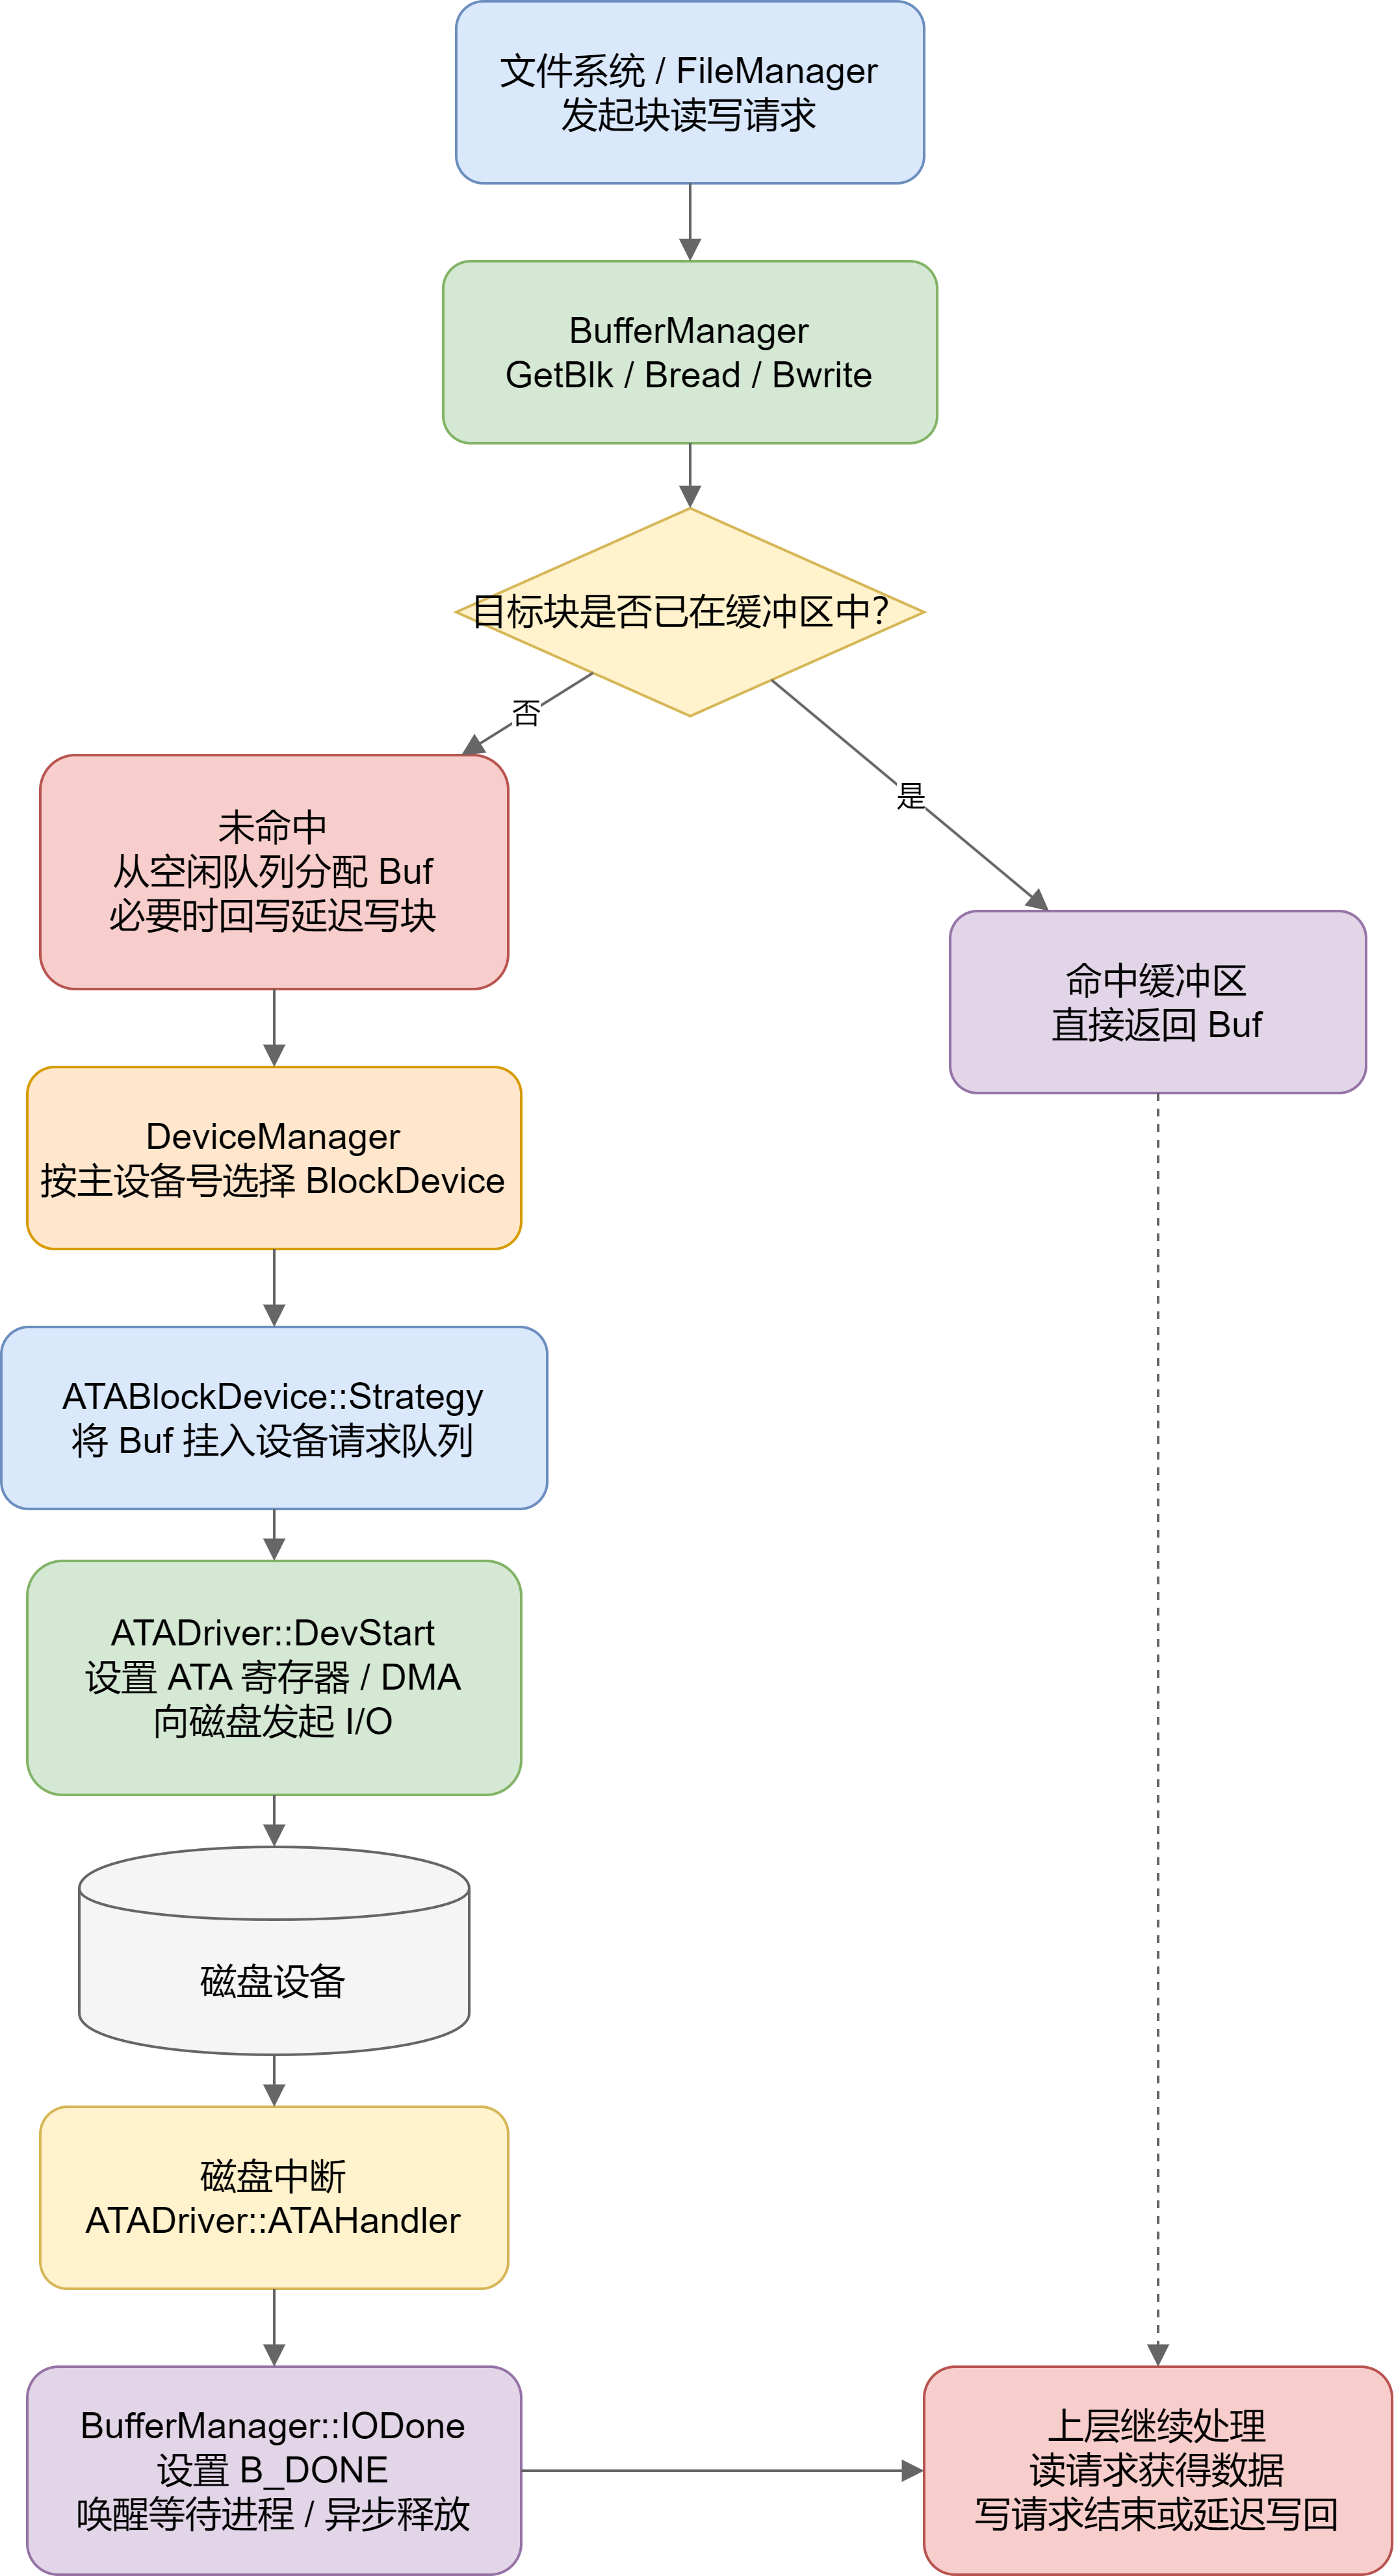
\includegraphics[height=0.62\textheight,keepaspectratio]{figures/2/3设备.png}
  \caption{缓冲区缓存与块设备访问流程图}
\end{figure}

\section{原系统存在的问题}

\subsection{IA32 架构的局限性}

Unix V6++原系统建立在 IA32 架构之上，其启动过程、分页机制、中断描述符表、任务状态段以及设备访问方式都与 x86 32 位平台紧密耦合。这种设计在早期教学环境中具有合理性，但随着现代硬件平台的发展，IA32 已逐渐退出主流，学生日常接触的处理器架构更多转向 x86-64 和 ARM，同时 RISC-V 也在教学和研究中迅速普及。此外，IA32 架构本身机制较为复杂，包含较多历史兼容性设计，例如分段与分页并存、实模式与保护模式、I/O 端口访问方式特殊等。这些特性虽然有助于理解传统 PC 体系结构，但也增加了教学负担，使学生难以抓住操作系统设计中的核心部分。因此，原系统在体系结构层面已难以完全适应当前操作系统教学的发展方向。

\subsection{C++实现的安全性与可维护性问题}

原系统虽然采用了 C++进行实现，在一定程度上利用了类和封装机制来组织代码，但其底层实现仍大量依赖裸指针、手工资源管理以及与硬件直接相关的低层操作。这些做法在系统软件中较为常见，但也带来了较大的安全风险。例如，内存分配与释放依赖程序员手工维护，文件对象和缓冲区对象的生命周期缺少编译期约束，容易出现悬垂指针、重复释放或越界访问等问题。同时，原系统代码中存在较多宏、全局对象以及跨模块隐式依赖，部分接口的职责边界不够清晰，给后续维护和扩展带来一定困难。随着系统功能逐步增加，这种以传统 C/C++风格为主的实现方式在可读性、可验证性和重构便利性方面都暴露出不足。

\subsection{原有实现与现代教学需求的不匹配}

从教学目标看，原系统在展示经典 Unix 核心思想方面具有明显优势，但在现代教学背景下也存在一定不足。首先，当前操作系统课程不仅关注经典机制本身，也逐渐重视现代指令集架构、内存安全、模块化设计和工程实践能力，而原系统在这些方面支持有限。其次，原系统的设备模型和驱动方式主要面向传统 PC 硬件，和现代

虚拟化环境下常见的 VirtIO 等机制存在较大差异。此外，随着 Rust 等现代系统编程语言的发展，教学中越来越强调如何在保证性

能的同时提升代码安全性和可维护性。原系统虽然适合作为经典实现样例，但若继续直接沿用，难以充分体现现代系统软件开发中的新方法与新工具。因此，有必要在保留其教学价值的基础上，对系统进行语言重构和体系结构迁移。

\section{重构与迁移目标}

本课题在语言层面的首要目标，是使用 Rust 对原系统中的核心模块进行重构，重点改善内存管理、文件系统及相关资源管理逻辑的安全性、效率与可维护性。在重构过程中，将尽量保持原系统的总体结构、主要数据关系和核心算法不变，以保证教学上的连续性，使学生仍能从中观察到传统 Unix 的基本设计思想。与此同时，Rust 的所有权、借用、智能指针和生命周期机制可用于替代原系统中大量依赖人工约束的资源管理方式。通过将原有裸指针操作封装在较小范围的 unsafe边界内，并在更高层提供类型安全接口，可以降低内存错误发生的可能性，并提高代码的可理解性和后续维护效率。在体系结构层面，本课题计划将系统从 IA32 平台迁移到 RISC-V 64 位平台。迁移目标包括使系统能够 QEMU 虚拟平台上启动运行，还包括对分页、中断、串口和块设备等关键机制完成适配。相较于 IA32，RISC-V 架构更加精简、开放，相关规范也更适合作为教学中的体系结构基础。通过迁移到 RISC-V，可以使系统更符合当前教学和研究环境的发展趋势，同时借助 Sv39 分页机制、特权级模型以及现代虚拟设备接口，向学生展示更具现实意义的操作系统底层实现路径。这样既保留了 Unix V6++的教学价值，也增强了系统的时代适应性。

\begin{table}[htbp]
  \centering
  \caption{重构前后目标对照表}
  \begin{tabular}{p{0.18\textwidth}p{0.34\textwidth}p{0.38\textwidth}}
    \toprule
    \textbf{对比维度} & \textbf{原系统} & \textbf{重构与迁移目标} \\
    \midrule
    指令集架构 & IA32 & RISC-V 64 \\
    实现语言 & C++ & Rust \\
    内存管理方式 & 页式管理较直接，分配算法较简化 & 建立更清晰、安全的内存抽象 \\
    文件系统 & 保留 Unix V6 风格，实现较传统 & 保留原有结构并提升安全性与可维护性 \\
    设备访问 & 基于 ATA 和传统 I/O 机制 & 适配更现代的设备接口与驱动模型 \\
    中断机制 & 依赖 IA32 中断体系 & 适配 RISC-V trap 机制 \\
    安全性 & 依赖人工保证，存在内存风险 & 利用所有权机制提升内存安全 \\
    可维护性 & 模块耦合较强，扩展不便 & 强化模块边界与类型化接口 \\
    教学适配性 & 偏重传统实现 & 兼顾经典原理与现代技术 \\
    \bottomrule
  \end{tabular}
\end{table}
